%%%%%%%%%%%%%%%%%%%%%%%%%%%%%%%%%%%%%%%%%%%%%%%%%%%%%%%%%%%%%%%%%%%%%%%
%%%% Содержание автореферата                                      %%%%
%%%%%%%%%%%%%%%%%%%%%%%%%%%%%%%%%%%%%%%%%%%%%%%%%%%%%%%%%%%%%%%%%%%%%%%

%%% Общая характеристика работы %%%
\pdfbookmark{Общая характеристика работы}{characteristic}
\section*{Общая характеристика работы}

\subsection*{Актуальность темы исследования}
\actualityText

\subsection*{Степень разработанности темы}
\degreeText

\subsection*{Цель работы}
\aimText

\subsection*{Задачи исследования}
\tasksText

\subsection*{Методология и методы исследования}
\methodsText

\subsection*{Объект исследования}
\objectText

\subsection*{Предмет исследования}
\subjectText

\subsection*{Научная новизна}
\noveltyText

\subsection*{Теоретическая значимость}
\theoreticalText

\subsection*{Практическая значимость}
\influenceText

\subsection*{Положения, выносимые на защиту}
\defpositionsText

\subsection*{Соответствие диссертации паспорту научной специальности}
\conformityText

\subsection*{Достоверность полученных результатов}
\reliabilityText

\subsection*{Апробация работы}
\probationText

\subsection*{Личный вклад автора}
\contributionText

\subsection*{Публикации}
\publicationsText

%%% Содержание работы %%%
\pdfbookmark{Содержание работы}{description}
\section*{Содержание работы}

Во \textbf{введении} обоснована актуальность темы диссертационной работы,
сформулирована цель исследования как повышение эффективности процессов
распознавания и~реидентификации людей в~информационно‑поисковых системах (ИПС)
в~режиме, близком к~реальному времени, и~определены задачи, решение которых
обеспечивает достижение поставленной цели. Приведены методология и~методы
исследования, раскрыты научная новизна, теоретическая и~практическая значимость,
сформулированы положения, выносимые на~защиту, а~также сведения об~апробации
и~внедрении результатов.

Отдельно подчёркнута специфика ReID в~ИПС как информационного процесса,
работающего с~видеопотоками и~характеризующегося информационной неопределённостью:
неполной доступностью модальностей (лицо/силуэт), вариативностью внешнего вида,
окклюзиями, изменением ракурса и~освещённости, а~также каскадным эффектом ошибок
последовательных этапов <<детектирование~→ извлечение признаков~→ принятие
решения>>. Это обосновывает необходимость комплексного подхода, в~котором
согласованно улучшаются ключевые этапы контура обработки данных.

\subsection*{Первая глава}

В~\textbf{первой главе} выполнен анализ теоретических основ распознавания
и~реидентификации личности и~рассмотрено место задачи ReID в~составе
информационно‑поисковых систем видеонаблюдения. Проведена систематизация
подходов к~распознаванию лица (классические методы выделения признаков и~снижения
размерности, методы детектирования и~сопоставления, современные нейросетевые
архитектуры и~функции потерь метрического обучения) и~подходов к~распознаванию
человека по~нелицевым признакам (силуэт, атрибуты внешнего вида, походка,
контекст сцены). Показано, что в~практических сценариях эксплуатации ни~одна
из~модальностей (только лицо или только тело) не~является гарантированно доступной
и~надёжной: лицо может отсутствовать из‑за окклюзии, низкого разрешения, малых
размеров в~кадре или неблагоприятного ракурса, а~признаки тела могут существенно
изменяться при смене одежды, позы и~условий наблюдения. Тем самым обоснована
необходимость многофакторных решений, интегрирующих комплементарные источники
признаков.

В~первой главе также рассмотрены современные постановки ReID и~person search
как задачи поиска объекта в~визуальном массиве при ограничениях по~времени ответа
и~вычислительным ресурсам. Показано, что типовые решения в~ИПС строятся как
последовательность взаимосвязанных информационных процессов: (1)~получение
видеоданных и~предобработка кадров, (2)~детектирование целевых объектов
(силуэт/лицо), (3)~ассоциация наблюдений во~времени (трекинг), (4)~формирование
признаковых представлений (эмбеддингов), (5)~интеграция нескольких источников
признаков и~принятие решения о~принадлежности наблюдаемого объекта одному
из~кандидатов в~базе, (6)~выдача результата (ID/ранжированный список/оценка
уверенности) и~протоколирование. Отмечено, что качество итогового поиска
и~реидентификации определяется согласованностью и~точностью всех перечисленных
процессов, а~ошибки на~ранних стадиях приводят к~каскадной деградации результата.

\begin{figure}[h]
\centering
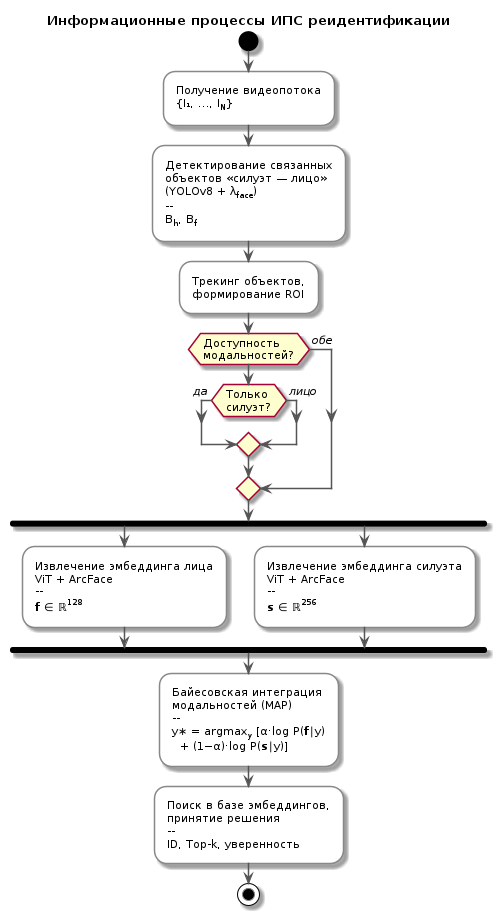
\includegraphics[width=0.9\textwidth]{images/1.png}
\caption{Схема информационных процессов ИПС реидентификации личности и~место
разработанных решений}
\label{fig:reid-scheme}
\end{figure}

Для формального описания контура обработки данных введены множества
и~отображения, задающие процесс распознавания/реидентификации в~ИПС.
Дано множество изображений (кадров) видеопотока:
\begin{equation}
    \mathcal{I}=\{I_i\}_{i=1}^{N},
    \label{eq:images}
\end{equation}
где каждое изображение $I_i$ содержит одного или нескольких людей.

Определены функции детектирования: функция детектирования силуэта (человека)
$D_h(\cdot)$, возвращающая множество ограничивающих рамок (силуэтов) $B_h$
для изображения~$I$; функция детектирования лица $D_f(\cdot)$, возвращающая
множество ограничивающих рамок лиц~$B_f$ для изображения~$I$ или пустое множество,
если лицо не~обнаружено; функция извлечения признаков (эмбеддинга) $\Phi(\cdot)$,
преобразующая детектированный объект (силуэт или лицо) в~вектор признаков заданной
размерности.

Необходимо определить правило объединения признаков двух модальностей,
позволяющее использовать доступные наблюдения в~условиях неполноты данных.
Вводится функция комбинирования $g(\cdot)$, формирующая комбинированный вектор
признаков~$\mathbf{z}$ на~основе вектора силуэта~$\mathbf{s}$ и~вектора
лица~$\mathbf{f}$:
\begin{equation}
    \mathbf{z}=g(\mathbf{s},\mathbf{f}).
    \label{eq:combination}
\end{equation}

Задача ИПС в~постановке первой главы формулируется как построение системы, которая
для каждого входного изображения~$I$ выполняет следующие шаги.

1)~Детектирование силуэта и~лица на~изображении~$I$:
\begin{equation}
    B_h=D_h(I),\quad B_f=D_f(I).
    \label{eq:detection}
\end{equation}

2)~Преобразование детектированных объектов в~векторы признаков с~помощью функции
$\Phi(\cdot)$. Для выбранных детекций (например, наиболее вероятных по~score либо
согласованных с~трекингом) вычисляются:
\begin{equation}
    \mathbf{s}=\Phi(\mathrm{ROI}_{human}),
    \label{eq:emb-human}
\end{equation}
\begin{equation}
    \mathbf{f}=\Phi(\mathrm{ROI}_{face}).
    \label{eq:emb-face}
\end{equation}

3)~Комбинирование векторов для получения интегрального описания наблюдаемого
объекта:
\begin{equation}
    \mathbf{z}=g(\mathbf{s},\mathbf{f}).
    \label{eq:combination-step}
\end{equation}

4)~Идентификация/реидентификация по~базе эмбеддингов (или по~индексу ИПС),
то~есть вычисление решающей функции $A(\cdot)$, которая по~вектору~$\mathbf{z}$
и~базе~$\mathrm{DB}$ возвращает идентификатор, оценку уверенности и/или
ранжированный список кандидатов.

Цель~--- минимизировать ошибку идентификации и~реидентификации при оптимальных
вычислительных затратах. Это требует согласованной оптимизации качества первичного
выделения объектов (детектирование), качества признакового описания (эмбеддинги)
и~корректности правила интеграции модальностей при принятии решения.

\subsection*{Вторая глава}

Во \textbf{второй главе} изложены теоретические результаты, составляющие
разработанную комплексную методику и~соответствующие трём положениям,
выносимым на~защиту. Глава структурирована по~логике
<<детектирование~→ формирование эмбеддингов~→ интеграция модальностей>>.

\textit{Первый результат} (положение~1) относится к~процессу детектирования
связанных объектов <<силуэт~--- лицо>>. Для усиления чувствительности
детектора к~ошибкам обнаружения лиц, ассоциированных с~силуэтом,
предложена модификация функции потерь YOLOv8: в~стандартный критерий
$\mathcal{L}_0$ введён дополнительный компонент $\mathcal{L}_{\text{face}}$
и~коэффициент~$\lambda_{\text{face}}$. Итоговая функция потерь имеет вид:
\begin{equation}
    \mathcal{L}=\mathcal{L}_0+\lambda_{\text{face}}\,
    \frac{1}{N}\sum_{i=1}^{N}\mathbb{I}_{\text{face}}(i)\,
    \mathcal{L}_{\text{face}}(i),
    \label{eq:loss}
\end{equation}
где $N$~--- число предсказаний, $\mathbb{I}_{\text{face}}(i)$~--- индикатор
наличия лица, $\mathcal{L}_{\text{face}}(i)$~--- штраф за~ошибку детекции лица.

\textit{Второй результат} (положение~2) относится к~процессу формирования
признаковых представлений (эмбеддингов) для лицевой и~силуэтной модальностей.
Предложен метод формирования дискриминативных эмбеддингов на~основе ансамбля
трансформерной архитектуры Vision Transformer (ViT) и~функции потерь ArcFace.
Метод обеспечивает формирование выраженных межклассовых границ
в~эмбеддинг‑пространстве и~позволяет использовать более дискриминативную
модальность (лицо) при её доступности либо компенсировать её отсутствие
силуэтной модальностью.

\textit{Третий результат} (положение~3) относится к~процессу интеграции
модальностей и~принятия решения в~задаче ReID. Предложена явная байесовская
модель интеграции эмбеддингов лица и~силуэта с~решающим правилом максимума
апостериорной вероятности (MAP). Задача распознавания моделируется как
статистическая классификация личности~$y$ по~двум наблюдениям: вектору признаков
лица~$\mathbf{f}$ и~вектору признаков силуэта~$\mathbf{s}$. Апостериорная
вероятность определяется по~теореме Байеса:
\begin{equation}
    P(y\mid \mathbf{f},\mathbf{s})=
    \frac{P(\mathbf{f}\mid y)\,P(\mathbf{s}\mid y)\,P(y)}
    {\sum\limits_{y'\in Y}P(\mathbf{f}\mid y')\,P(\mathbf{s}\mid y')\,P(y')}.
    \label{eq:bayes}
\end{equation}

В~условиях непредвзятой идентификации правило принятия решения имеет вид
MAP‑критерия:
\begin{equation}
    y^*=\arg\max\limits_{y\in Y}
    \left[\log P(\mathbf{f}\mid y)+\log P(\mathbf{s}\mid y)\right].
    \label{eq:map}
\end{equation}

Таким образом, во~второй главе сформирована единая логическая цепочка:
модифицированный критерий обучения детектора повышает качество извлечения
ROI~лица (положение~1); метод формирования дискриминативных эмбеддингов
обеспечивает устойчивые векторные представления (положение~2); байесовская
модель интеграции и~MAP‑решение обеспечивают корректное объединение модальностей
и~принятие решения в~условиях неполноты данных (положение~3).

\subsection*{Третья глава}

В~\textbf{третьей главе} приведена экспериментальная проверка разработанных
решений. Эксперименты структурированы в~соответствии с~тремя положениями,
выносимыми на~защиту. Для оценки ReID использованы репрезентативные наборы
данных CUHK03, Market‑1501 и~MARS.

\textit{Эксперименты по~положению~1.} Выполнена подготовка данных и~обучение
модифицированной модели YOLOv8. Экспериментально исследовано влияние коэффициента
$\lambda_{\text{face}}$ на~показатели качества детекции по~классам <<face>>
и~<<силуэт>>. Варьирование $\lambda_{\text{face}}$ выполнялось в~диапазоне
от~0.1 до~2.7. Экспериментально установлено, что значения $\lambda_{\text{face}}$
в~диапазоне 2.0--2.7 обеспечивают максимальные показатели по~детекции лиц
при отсутствии деградации по~классу <<силуэт>>, что подтверждает работоспособность
предложенной модификации критерия обучения.

\textit{Эксперименты по~положению~2.} Проведена качественная оценка эмбеддингов,
сформированных предложенным методом для лицевой и~силуэтной модальностей.
Для анализа структуры эмбеддинг‑пространств использована визуализация методом
t‑SNE. Визуальный анализ подтверждает, что дискриминативные эмбеддинги
формируют более выраженную кластеризацию по~идентичностям и~позволяют уменьшить
пересечения классов в~пространстве признаков.

\textit{Эксперименты по~положению~3.} Выполнена экспериментальная оценка
качества многоклассовой классификации в~задаче ReID при использовании байесовской
интеграции модальностей. По~результатам вычислительных экспериментов на~наборе
CUHK03 получены значения: Precision~--- 95.65\%, Recall~--- 95.54\%,
F1‑мера~--- 94.31\%, Accuracy~--- 93.42\%. Для объективного сравнения
с~современными решениями выполнена оценка по~метрике mean average precision~(mAP)
на~наборах данных CUHK03, Market‑1501 и~MARS. Результаты подтверждают
конкурентоспособность предложенного метода интеграции по~mAP (95.65\%~/~98.3\%~/~89.2\%
для CUHK03~/~Market‑1501~/~MARS соответственно)

\FloatBarrier

%%% Заключение %%%
\pdfbookmark{Заключение}{conclusion}
\section*{Заключение}

Показано, что решена научно‑техническая задача повышения точности реидентификации
людей в~ИПС в~условиях изменяющихся факторов наблюдения за~счёт: (1)~модификации
критерия обучения детектора связанных объектов <<силуэт--лицо>>, (2)~формирования
дискриминативных эмбеддингов лица и~силуэта, (3)~вероятностной интеграции
модальностей и~принятия решения по~MAP‑критерию. Экспериментально подтверждено,
что предложенная комплексная методика обеспечивает повышение устойчивости
и~качества реидентификации по~сравнению с~раздельным использованием модальностей
и~с~простыми схемами линейного объединения, а~также сохраняет применимость
к~режимам работы, близким к~реальному времени

%%% Список публикаций %%%
\pdfbookmark{Список публикаций}{publications}
\section*{Список публикаций по теме диссертации}

\subsection*{Статьи в журналах, рекомендованных ВАК}

\begin{enumerate}
    \item \textbf{Фамилия~И.\,О.} Название статьи~// Название журнала. 2023.
          Т.~1, №~1. С.~1--10.
    \item \textbf{Фамилия~И.\,О.}, Соавтор~И.\,О. Название статьи~//
          Название журнала. 2024. Т.~2, №~2. С.~11--20.
\end{enumerate}

\subsection*{Публикации в других изданиях}

\begin{enumerate}[resume]
    \item \textbf{Фамилия~И.\,О.} Название доклада~// Труды конференции.
          Город, 2023. С.~100--105.
\end{enumerate}
